\documentclass[tikz]{standalone}

\usetikzlibrary{arrows.meta,positioning}

\begin{document}
	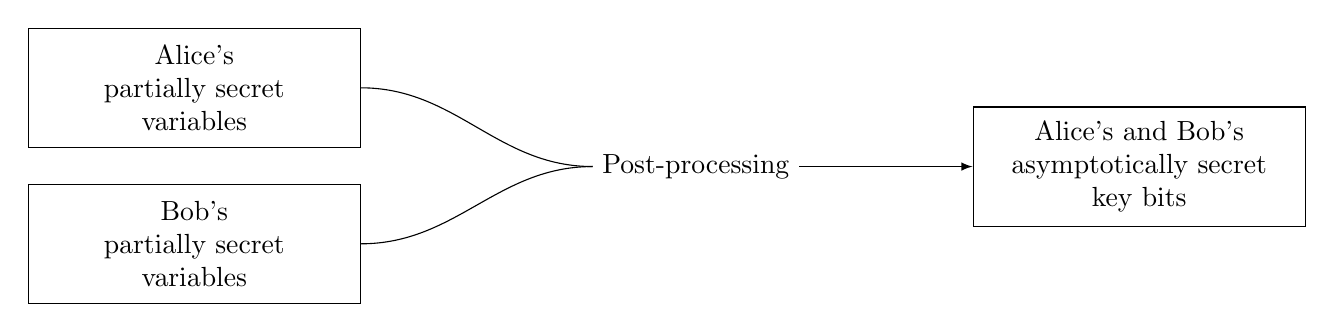
\begin{tikzpicture}[
		node distance=3ex,
		arrow/.style={-latex},
		block/.style={draw, minimum height=10ex, minimum width=12em, align=center},
	]
		\node (av) [block] {Alice's\\partially secret\\variables};
		\node (bv) [block, below=of av] {Bob's\\partially secret \\variables};
		\node (sb) at (12,-1) [block] {Alice's and Bob's\\asymptotically secret\\key bits};
		\node (n) at ([xshift=-10em]sb.west) {Post-processing};
		
		\draw (av.east) to[out=0, in=180] (n);
		\draw (bv.east) to[out=0, in=180] (n);
		\draw[arrow] (n) -- (sb.west);
	\end{tikzpicture}
\end{document}
